% !TEX root = ../Main.tex
\chapter{正四面体与正三棱锥}

正四面体四个面都是全等的正三角形，是最对称的立体。它同时有外接球与内切球，且两球\textbf{同心}。下面用三种方法求半径，再推广到一般正三棱锥。

\section{正四面体的外接球与内切球}

设正四面体棱长为 $a$。底面是边长 $a$ 的正三角形，其中心 $O'$ 到顶点 $B$ 的距离 $O'B=\dfrac{a}{\sqrt3}$，顶点 $P$ 到底面的高
\[
h=\sqrt{a^2-\Big(\tfrac{a}{\sqrt3}\Big)^2}=\sqrt{a^2-\tfrac{a^2}{3}}=\frac{\sqrt6}{3}a.
\]
由对称性，外接球球心、内切球球心都在 $P$ 与底面中心 $O'$ 的连线上，两球同心。

\begin{center}
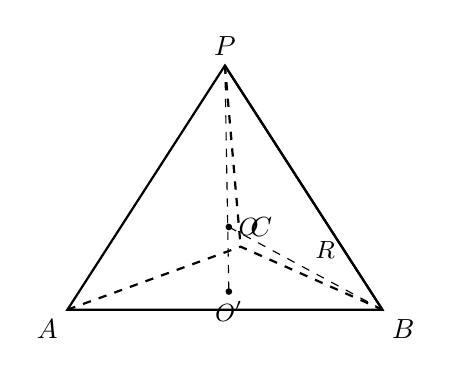
\begin{tikzpicture}[scale=1]
    \coordinate (P) at (0,2.6);
    \coordinate (A) at (-2,-0.5);
    \coordinate (B) at (2,-0.5);
    \coordinate (C) at (0.2,0.3);
    \draw[thick] (P) -- (A) -- (B) -- cycle;
    \draw[thick] (P) -- (B);
    \draw[thick, dashed] (A) -- (C) -- (B);
    \draw[thick, dashed] (P) -- (C);
    \coordinate (Op) at (0.05,-0.27);
    \coordinate (O) at (0.05,0.55);
    \draw[dashed] (P) -- (Op);
    \fill (O) circle (1.2pt) node[right] {\small $O$};
    \fill (Op) circle (1.2pt) node[below] {\small $O'$};
    \draw[dashed] (O) -- (B) node[midway,above right]{\small $R$};
    \node at (P) [above] {$P$};
    \node at (A) [below left] {$A$};
    \node at (B) [below right] {$B$};
    \node at (C) [above right] {$C$};
\end{tikzpicture}
\end{center}

\ex[几何法]{
    求正四面体外接球半径 $R$。
}

\sol{
    球心 $O$ 在 $PO'$ 上。$O$ 到顶点 $P$ 距离 $=R$、$O$ 到 $O'$ 距离 $=h-R$，$O$ 到底面顶点 $B$ 距离也是 $R$，而 $O'B=\tfrac{a}{\sqrt3}$：
    \[
    R^2=(h-R)^2+\Big(\tfrac{a}{\sqrt3}\Big)^2
    =h^2-2hR+R^2+\tfrac{a^2}{3}.
    \]
    约去 $R^2$，代入 $h=\tfrac{\sqrt6}{3}a$（$h^2=\tfrac{2a^2}{3}$）：
    \[
    2hR=h^2+\tfrac{a^2}{3}=\tfrac{2a^2}{3}+\tfrac{a^2}{3}=a^2
    \ \Longrightarrow\ R=\frac{a^2}{2h}=\frac{a^2}{2\cdot\frac{\sqrt6}{3}a}=\frac{\sqrt6}{4}a.
    \]
    球心到底面的距离 $r=h-R=\dfrac{\sqrt6}{3}a-\dfrac{\sqrt6}{4}a=\dfrac{\sqrt6}{12}a$，由两球同心，这就是内切球半径。于是
    \[
    R=\frac{\sqrt6}{4}a,\qquad r=\frac{\sqrt6}{12}a,\qquad R+r=h,\quad R=3r.
    \]
}

\ex[体积分割法]{
    用 $V=\tfrac13 S_{\text{表}}r$ 求内切球半径。
}

\sol{
    四个面都是边长 $a$ 的正三角形，面积都记作 $S=\tfrac{\sqrt3}{4}a^2$。把正四面体沿内心切成四个小棱锥，各以一个面为底、高为 $r$：
    \[
    V=\frac13 S\,r\times4=\frac43 S\,r.
    \]
    另一方面，以底面为底、高为 $h$：$V=\dfrac13 S h$。两式相等得 $h=4r$，即
    \[
    r=\frac{h}{4}=\frac{1}{4}\cdot\frac{\sqrt6}{3}a=\frac{\sqrt6}{12}a,
    \qquad R=3r=\frac{\sqrt6}{4}a.
    \]
    与几何法一致。$h=4r$（等价 $R=3r$）是正四面体最好记的关系。
}

\ex[嵌入正方体]{
    把正四面体嵌进正方体，用空间对角线求 $R$。
}

\sol{
    取正方体的四个交错顶点，连成的就是一个正四面体，它的棱恰是正方体的\textbf{面对角线}。设正方体棱长 $s$，则正四面体棱长 $a=\sqrt2\,s$。正四面体与正方体\textbf{共外接球}，球心为正方体中心，直径即空间对角线 $\sqrt3\,s$：
    \[
    2R=\sqrt3\,s=\sqrt3\cdot\frac{a}{\sqrt2}=\frac{\sqrt6}{2}a
    \ \Longrightarrow\ R=\frac{\sqrt6}{4}a.
    \]
    三种方法结果一致。
}

\begin{center}
\begin{tikzpicture}[scale=1.1]
    \draw[thick] (0,0) -- (2,0) -- (2,2) -- (0,2) -- cycle;
    \draw[thick] (0.7,0.7) -- (2.7,0.7) -- (2.7,2.7) -- (0.7,2.7) -- cycle;
    \draw[thick] (0,0) -- (0.7,0.7);
    \draw[thick] (2,0) -- (2.7,0.7);
    \draw[thick] (2,2) -- (2.7,2.7);
    \draw[thick] (0,2) -- (0.7,2.7);
    \coordinate (V1) at (0,0);
    \coordinate (V2) at (2,2);
    \coordinate (V3) at (2.7,0.7);
    \coordinate (V4) at (0.7,2.7);
    \draw[thick, red] (V1)--(V2) (V1)--(V3) (V1)--(V4) (V2)--(V3) (V2)--(V4) (V3)--(V4);
    \node at (1.35,-0.6) {\small 正方体里的正四面体：棱即面对角线};
\end{tikzpicture}
\end{center}

\section{一般正三棱锥}

正三棱锥的顶点 $P$ 在底面正三角形中心 $O'$ 正上方，但侧棱与底边不一定相等，所以高 $h$ 是独立给的。球心仍在 $PO'$ 这条轴上，几何法照搬：设底边长 $a$（底面外接圆半径 $\tfrac{a}{\sqrt3}$）、高 $h$，
\[
R^2=(h-R)^2+\Big(\tfrac{a}{\sqrt3}\Big)^2
\ \Longrightarrow\
R=\frac{h^2+\frac{a^2}{3}}{2h}.
\]

\state{轴上球心的垂线模型}{
    只要顶点 $P$ 在底面外接圆圆心 $O'$ 正上方、距离为 $h$，底面外接圆半径为 $r$，则球心在 $PO'$ 上，由 $R^2=(h-R)^2+r^2$ 得
    \[
    R=\frac{h^2+r^2}{2h}.
    \]
}
